\documentclass[10pt]{article}
\usepackage{icmlko}

\icmlmeta{IP 파운데이션 월드모델}{38}{대상을 위해 배선하면 출처를 잃는다}{싼 판정 기준으로 배선을 전수 탐색했더니 이득이 상쇄됐다 --- 자기 상관을 올리면 대상으로선 좋아지고 출처로선 나빠진다}

\begin{document}

\twocolumn[
\icmlheader

\begin{abstract}
노트 37이 판정을 싸게 만들었다. 전이 상관은 대상의 \emph{인자 공간} 자기 상관과
같으므로($+$0.993) 배선 후보를 열두 셀 순열 검정 없이 도메인 하나 안에서 평가할
수 있다. 그래서 네 도메인의 배선을 좌표 상승법으로 전수 탐색했다. 후보를 많이
보고 최댓값을 고르면 낙관적이므로 --- 노트 4의 헤드라인을 철회하게 만든 그
선택 편향 --- 반복 교차검증, 확인용 씨앗, 독립 측정 세 가지로 막았다. 결과는
\textbf{게임 $+$0.060, 아이돌 $+$0.035}(확인 씨앗 기준 순증)이고 팝업과 도서는
현행 배선이 이미 지역 최적이었다. \textbf{그런데 열두 셀에서 확인하니 이득이
$+$0.0529에서 $+$0.0536으로 거의 오르지 않았다.} 셀을 하나씩 보니 방향이
갈렸다 --- 게임을 \emph{대상}으로 한 세 셀은 전부 좋아지고 \emph{출처}로 한 두
셀은 나빠졌다. 도메인별로 두 역할을 나눠 재니 관계가 선명하다.
\textbf{인자 공간 자기 상관의 변화는 대상으로서의 전이와 $r=+$0.966,
출처로서의 전이와 $r=-$0.870이다.} 자기 라벨에 맞춰 배선할수록 그 인자 공간은
도메인 특수적이 되고, 남에게 빌려줄 때 덜 일반적이 된다. 노트 33의 ``출처 선택은
무의미하다''를 정정해야 한다 --- 관측된 범위에서 무관했던 것과 개입했을 때
무관한 것은 다르다. 아이돌만 두 역할이 함께 올라 채택했고(열두 셀 이득
$+$0.0547) 게임 배선은 상충이 상쇄해 보류했다.
\end{abstract}
]

\section{싼 판정으로 전수 탐색}

노트 37의 부산물이 컸다. 인자 공간 자기 상관은 그 도메인 안에서만 계산되므로,
배선 후보를 평가할 때 전이를 돌릴 필요가 없다. 5폴드 교차검증 한 번이면 된다.

그래서 좌표 상승법을 짰다. 슬롯을 하나씩 돌며 후보를 전부 시험해 가장 좋은
것으로 바꾸고, 한 바퀴에 아무 변화도 없으면 멈춘다.

\paragraph{싼 판정은 새 위험을 낳는다}
후보를 많이 보고 최댓값을 고르면 그 최댓값은 낙관적이다. 노트 4의 헤드라인을
철회하게 만든 선택 편향이 그대로 재현될 수 있다. 세 가지로 막았다.

\begin{itemize}[leftmargin=1.1em,itemsep=0.15em]
\item \textbf{반복 교차검증} --- 씨앗 다섯 개의 평균으로 고른다.
\item \textbf{확인용 씨앗} --- 고를 때 쓰지 않은 씨앗 다섯 개로 승자를 다시 잰다.
      두 값의 차이가 편향의 크기이며 아래 표에 그대로 적는다.
\item \textbf{독립 측정} --- 최종 승자만 열두 셀 순열 검정으로 확인한다.
\end{itemize}

\begin{figure}[t]
\centering
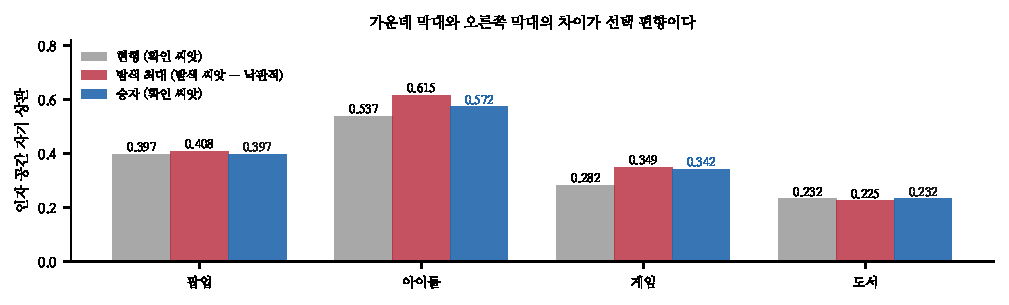
\includegraphics[width=\textwidth]{figs/search.pdf}
\caption{배선 탐색 결과. 가운데와 오른쪽 막대의 차이가 선택 편향이다.}
\end{figure}

\begin{table}[t]
\centering\tsize
\caption{탐색 결과. 편향 $=$ 탐색 최대 $-$ 확인 씨앗.}
\begin{tabular}{lrrrr}
\toprule
도메인 & 현행 & 탐색 최대 & 확인 & 편향 \\
\midrule
팝업 & $+$0.397 & $+$0.408 & $+$0.397 & $+$0.011 \\
아이돌 & $+$0.537 & $+$0.615 & $+$0.572 & \textbf{$+$0.043} \\
게임 & $+$0.282 & $+$0.349 & $+$0.342 & $+$0.007 \\
도서 & $+$0.232 & $+$0.225 & $+$0.232 & $-$0.007 \\
\bottomrule
\end{tabular}
\end{table}

팝업과 도서는 좌표 상승이 한 칸도 움직이지 못했다 --- 현행 배선이 이미 지역
최적이다. 아이돌은 편향이 $+$0.043으로 순증($+$0.035)과 비슷한 크기라 조심해야
하고, 게임은 편향이 $+$0.007로 작아 믿을 만하다.

\begin{table}[t]
\centering\tsize
\caption{탐색이 찾은 배선 변경.}
\begin{tabular}{ll}
\toprule
도메인 & 변경 \\
\midrule
아이돌 & 입장 허들 $\leftarrow$ 앨범 정가 \\
     & 굿즈 규모 $\leftarrow$ 앨범 버전 수(정가 분리) \\
게임 & 타깃 폭 $\leftarrow$ 지원 언어 수 \\
     & 굿즈 규모 $\leftarrow$ Steam 기능 수 \\
\bottomrule
\end{tabular}
\end{table}

아이돌 변경은 한 축에 묶여 있던 정가와 버전 수를 떼어낸 것이다. 둘의 상관이
$+$0.198로 낮아 서로 다른 것을 재고 있었는데 한 축에 넣어 둘 다 흐렸다.

\section{그런데 열두 셀에서는 안 올랐다}

\begin{table}[t]
\centering\tsize
\caption{독립 측정. 탐색에 쓰지 않은 열두 셀 순열 검정.}
\begin{tabular}{lrr}
\toprule
설정 & 유의 & 평균 이득 \\
\midrule
현행 & 10/12 & $+$0.0529 \\
탐색 승자(둘 다) & 10/12 & $+$0.0536 \\
게임만 & 10/12 & $+$0.0528 \\
\textbf{아이돌만} & \textbf{10/12} & \textbf{$+$0.0547} \\
\bottomrule
\end{tabular}
\end{table}

인자 공간 자기 상관이 게임에서 $+$0.060 올랐는데 전체 이득은 1\%밖에 안 올랐다.
게임 배선만 적용하면 오히려 미세하게 내려간다.

셀을 하나씩 보니 방향이 갈렸다.

\begin{table}[t]
\centering\tsize
\caption{게임 배선을 바꿨을 때 게임이 낀 셀들.}
\begin{tabular}{lrrl}
\toprule
셀 & 현행 & 변경 후 & \\
\midrule
팝업 $\to$ 게임 & $-$0.0275 & $-$0.0323 & 개선 \\
아이돌 $\to$ 게임 & $-$0.0067 & $-$0.0082 & 개선 \\
도서 $\to$ 게임 & $-$0.0267 & $-$0.0289 & 개선 \\
\midrule
게임 $\to$ 팝업 & $-$0.1042 & $-$0.0971 & \textbf{악화} \\
게임 $\to$ 도서 & $-$0.0289 & $-$0.0151 & \textbf{악화} \\
\bottomrule
\end{tabular}
\end{table}

게임을 대상으로 한 셋은 전부 좋아지고 출처로 한 둘은 나빠진다.

\section{두 역할이 반대로 움직인다}

도메인마다 두 역할을 나눠 평균을 냈다.

\begin{figure}[t]
\centering
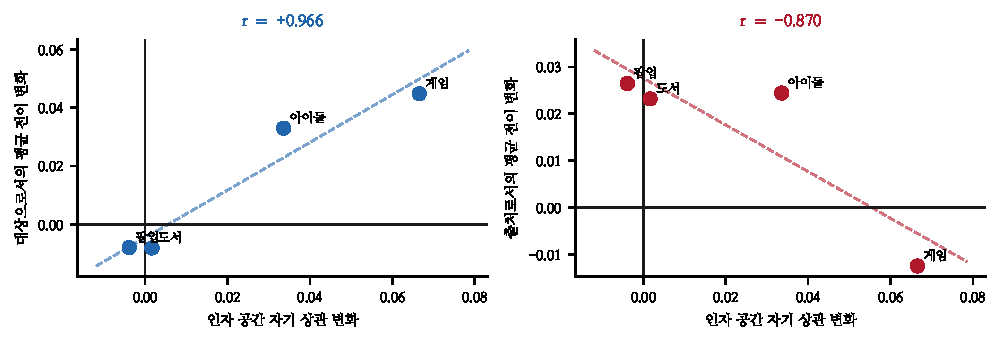
\includegraphics[width=\textwidth]{figs/tradeoff.pdf}
\caption{인자 공간 자기 상관 변화와 두 역할의 전이 변화.}
\end{figure}

\begin{table}[t]
\centering\tsize
\caption{탐색 전후. 화살표는 변화 방향이다.}
\begin{tabular}{lrrr}
\toprule
도메인 & 자기 상관 & 대상으로 & 출처로 \\
\midrule
팝업 & $+$0.408$\to$$+$0.404 & $+$0.462$\to$$+$0.454 & $+$0.411$\to$$+$0.437 \\
아이돌 & $+$0.582$\to$$+$0.615 & $+$0.657$\to$$+$0.690 & $+$0.332$\to$$+$0.357 \\
게임 & $+$0.282$\to$$+$0.349 & $+$0.296$\to$$+$0.341 & $+$0.465$\to$$+$0.452 \\
도서 & $+$0.224$\to$$+$0.225 & $+$0.253$\to$$+$0.245 & $+$0.459$\to$$+$0.482 \\
\bottomrule
\end{tabular}
\end{table}

\begin{table}[t]
\centering\tsize
\caption{자기 상관 변화가 무엇을 예측하나(네 도메인).}
\begin{tabular}{lr}
\toprule
& 자기 상관 변화와의 상관 \\
\midrule
\textbf{대상으로서의 전이 변화} & \textbf{$+$0.966} \\
\textbf{출처로서의 전이 변화} & \textbf{$-$0.870} \\
\bottomrule
\end{tabular}
\end{table}

\claimx{한 도메인의 인자 공간 자기 상관을 올리면 그 도메인은 대상으로서
좋아지고($r=+$0.966) 출처로서 나빠진다($r=-$0.870). 자기 라벨에 맞춰 배선할수록
인자 공간이 도메인 특수적이 되어 남에게 빌려줄 때 덜 일반적이다.}{네 점으로 잰
상관이므로 도메인을 더 넣었을 때 부호가 유지되는지 봐야 한다. 특히 두 역할이
함께 오르는 배선이 여럿 나오면 상충이 아니라 배선의 질 문제다.}

\begin{figure}[t]
\centering
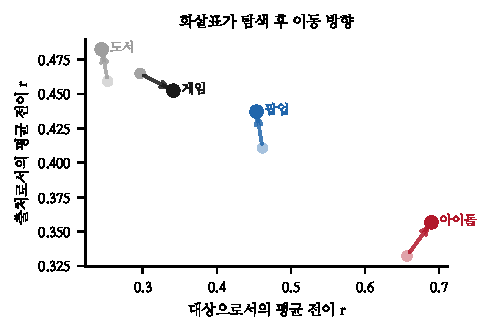
\includegraphics[width=\columnwidth]{figs/roles.pdf}
\caption{두 역할 평면에서의 이동. 대체로 오른쪽 아래나 왼쪽 위로 움직인다.}
\end{figure}

\section{노트 33을 정정한다}

노트 33은 이렇게 썼다 --- ``출처 자기 상관이 $-$0.436, 출처 표본 수가 $+$0.360,
출처 축 수가 $-$0.243이다. 어느 것도 전이 성능을 설명하지 못한다. \textbf{출처
선택은 무의미하다}.''

관측으로는 맞았다. 여섯(뒤에 열둘) 셀에서 출처 쪽 어떤 특성도 전이를 설명하지
않았다. 그러나 그것은 \emph{주어진 배선들을 관찰한} 결과다. 배선에 \emph{개입}하면
출처 성능이 체계적으로 움직인다.

\begin{quote}\fontsize{9.5}{11.5}\selectfont
관측에서 상관이 없다는 것과 개입해도 효과가 없다는 것은 다른 주장이다. 노트
33은 앞의 것을 재고 뒤의 것을 결론지었다. \textbf{출처 선택은 무의미하지만
출처 배선은 유의미하다.}
\end{quote}

이것은 왜 노트 33에서 출처 자기 상관이 \emph{음의} 상관($-$0.436, 나중에
$-$0.309)을 보였는지도 설명한다. 각 도메인의 배선은 그 도메인의 라벨을 보며
다듬어졌고, 잘 다듬어진 도메인일수록 특수화돼 출처로서 불리했던 것이다.

\section{채택}

아이돌만 두 역할이 함께 올랐다(대상 $+$0.657$\to+$0.690, 출처
$+$0.332$\to+$0.357). 채택했다.

게임 배선은 대상 $+$0.045, 출처 $-$0.013으로 상충이 상쇄한다. 게임은 표본이
482건으로 가장 크고 출처로 자주 쓰이므로 보류했다.

\begin{table}[t]
\centering\tsize
\caption{아이돌 배선 채택 후. 공통 축 셋, 성분 둘.}
\begin{tabular}{lrr}
\toprule
셀 & $\Delta$ & p \\
\midrule
팝업 $\to$ 아이돌 & $-$0.1019 & 0.0000 \\
팝업 $\to$ 게임 & $-$0.0268 & 0.0070 \\
팝업 $\to$ 도서 & $-$0.0250 & 0.0183 \\
아이돌 $\to$ 팝업 & $-$0.0926 & 0.0137 \\
아이돌 $\to$ 게임 & $-$0.0042 & 0.2917 \\
아이돌 $\to$ 도서 & $+$0.0064 & 0.5120 \\
게임 $\to$ 팝업 & $-$0.1034 & 0.0000 \\
게임 $\to$ 아이돌 & $-$0.0920 & 0.0000 \\
게임 $\to$ 도서 & $-$0.0289 & 0.0000 \\
도서 $\to$ 팝업 & $-$0.0877 & 0.0000 \\
도서 $\to$ 아이돌 & $-$0.0745 & 0.0000 \\
도서 $\to$ 게임 & $-$0.0263 & 0.0003 \\
\bottomrule
\end{tabular}
\end{table}

\paragraph{제품 쪽에는 좋은 소식이다}
팝업은 대상으로만 쓴다 --- 다른 도메인에서 배워 팝업을 예측하는 것이 목적이고
팝업으로 남을 가르칠 일이 없다. 그러니 상충이 문제가 되지 않는다. 팝업의 인자
공간 자기 상관만 올리면 된다. 다만 이번 탐색에서 팝업은 한 칸도 못 움직였다.

\section{한계}

\begin{itemize}[leftmargin=1.1em,itemsep=0.15em]
\item 상충 상관을 네 점으로 쟀다. 도메인이 넷뿐이라 $+$0.966과 $-$0.870 모두
      점 하나에 크게 흔들린다.
\item 아이돌 편향($+$0.043)이 순증($+$0.035)보다 크다. 열두 셀 확인에서
      $+$0.0547로 올랐으므로 채택했지만 그 차이도 작다.
\item 좌표 상승법은 지역 최적만 찾는다. 슬롯 둘을 동시에 바꿔야 좋아지는 배선은
      못 찾는다.
\item 팝업이 한 칸도 못 움직인 것이 진짜 최적이어서인지 후보가 빈약해서인지
      모른다. 팝업 후보는 사람이 매긴 열 속성뿐이다.
\item 게임 배선을 보류했지만, 팝업이 유일한 실제 대상이라면 게임을 출처로서
      최적화하는 것이 옳을 수도 있다. 그 방향의 탐색은 하지 않았다.
\end{itemize}

\section{다음}

\begin{enumerate}[leftmargin=1.3em,itemsep=0.15em]
\item 출처 전용 목적함수 --- 팝업을 대상으로 고정하고 나머지 셋을 출처로서
      최적화한다. 상충의 반대편을 쓰는 것이다.
\item 팝업 축 후보를 늘린다 --- 기획서에서 새 속성을 태깅하거나 물리적 계측치를
      더한다.
\item 상충의 메커니즘 --- 인자 적재가 어떻게 특수화되는지 직접 본다.
\item 도메인을 다섯째로 늘려 상충 상관을 다시 잰다.
\end{enumerate}

\vspace{0.6em}
\hrule height 0.3pt
\vspace{0.5em}
{\footnotesize
\textbf{참고문헌}\\[0.3em]
Ben-David, S. et al. (2010). A theory of learning from different domains.
\emph{Machine Learning}, 79(1--2), 151--175.\\[0.15em]
Standley, T. et al. (2020). Which tasks should be learned together in multi-task
learning? \emph{ICML}, 9120--9132.\\[0.15em]
Pearl, J. (2009). \emph{Causality: Models, Reasoning, and Inference}, 2nd ed.
Cambridge University Press.\\[0.15em]
Cawley, G. C., Talbot, N. L. C. (2010). On over-fitting in model selection and
subsequent selection bias in performance evaluation. \emph{JMLR}, 11, 2079--2107.\\[0.15em]
Schönemann, P. H. (1966). A generalized solution of the orthogonal Procrustes
problem. \emph{Psychometrika}, 31(1), 1--10.
}

\end{document}
